\documentclass{article}
% Choose a conveniently small page size
% PACKAGES
\usepackage[margin = 1in]{geometry}
\usepackage{amsfonts}
\usepackage{amsmath}
\usepackage{amssymb}
\usepackage{multicol}
\usepackage{graphicx}
\usepackage{float}
\usepackage{xcolor}
\usepackage{amsthm}
\usepackage{dsfont}
\usepackage{hyperref}
\usepackage{float}

% MACROS
% Set Theory
\def\N{\mathbb{N}}
\def\R{\mathbb{R}}
\def\C{\mathbb{C}}
\def\Z{\mathbb{Z}}
%\def\^{\hat}
\def\-{\vec}
\def\d{\partial}
\def\!{\boldsymbol}
\def\X{\times}
%\def\-{\bar}
\def\bf{\textbf}
\def\l{\left}
\def\r{\right}
\title{Weekly Report 2}
\author{Damien}
\begin{document}
\maketitle
% \newpage
\section{Progress}
I made more progress towards solving problem 5.1.1. However, the results are still not satisfactory. My theoretical understanding of the Lax-Friedrichs sweeping method is still the same as it was last week. However, I found that I was handling the ghost cells incorrectly. In addition, there was a small mistake in my implementation of the flux. The method still did not work so I ran some tests to diagnose what is going wrong. All of the following simulations are for $\beta = \frac{1}{2}$. I tried tests on $\beta=2$, but they suffer from an identical problem, so I did not include them in this report. I also ran some tests by using the WENO fluxes in a time-stepping method. However, these results with the updated ghost cells look nearly identical to the plots I gave last week and I did not include them in this report.
\subsection{Ghost Cells}
In my previous report I set the ghost cells to all have zero for problem 5.1.1. I read through Kao et al. and found that they simply set the values at the ghost points to the values of the exact solution to make things easier. With 104 grid cells (including four ghost cells) the initial conditions appear as follows.
\begin{figure*}[h]
    \centering
    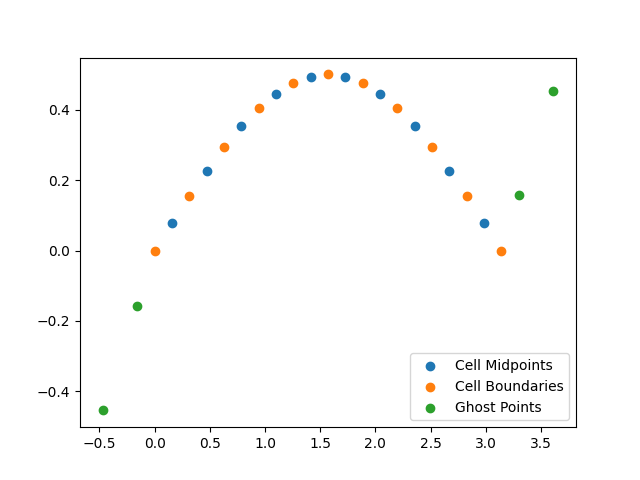
\includegraphics[width=0.5\textwidth]{imgs/ics.png}
    \caption{This figure shows how the grid cells are distributed for the third order WENO scheme. The x-axis is space}
    \label{fig:ics}
\end{figure*}
\subsection{Third order Lax–Friedrichs WENO sweeping method}
I implemented the method that I discussed last week. I realized that decreasing the value of $\sigma$ to $20$ helped improve the convergence... somewhat. 
\begin{figure*}[t!]
    \centering
    \begin{minipage}{.48\textwidth}
        \centering
        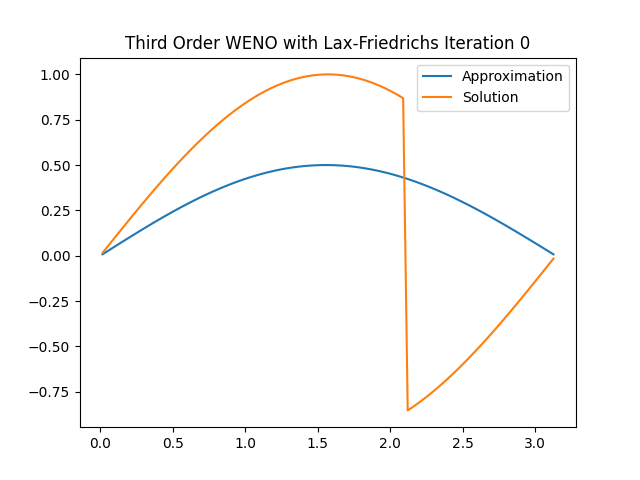
\includegraphics[width=0.9\linewidth]{imgs/output_weno3_lf/plot_0.png}
        %   \caption{figure}{A figure}
        % \label{fig:test1}
    \end{minipage}%
    \begin{minipage}{.48\textwidth}
        \centering
        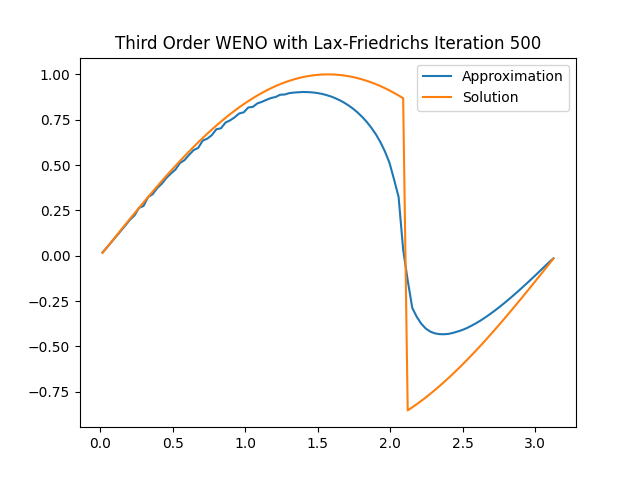
\includegraphics[width=0.9\linewidth]{imgs/output_weno3_lf/plot_500.png}
        %   \caption{figure}{Another figure}
        % \label{fig:test2}
    \end{minipage}
\par\bigskip
    \begin{minipage}{.48\textwidth}
        \centering
        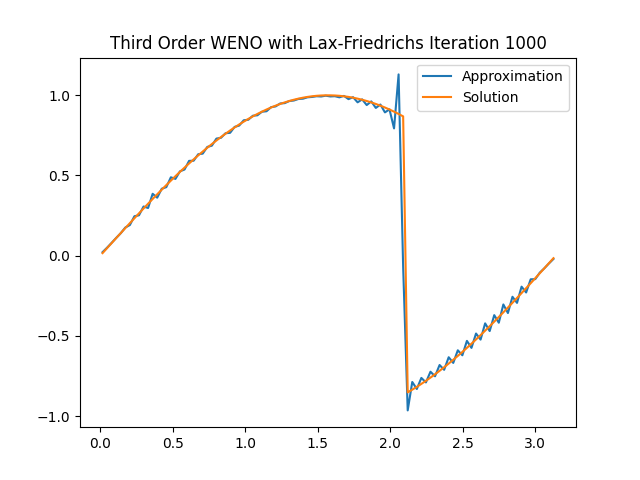
\includegraphics[width=0.9\linewidth]{imgs/output_weno3_lf/plot_1000.png}
        %   \caption{figure}{A figure}
        % \label{fig:test1}
    \end{minipage}%
    \begin{minipage}{.48\textwidth}
        \centering
        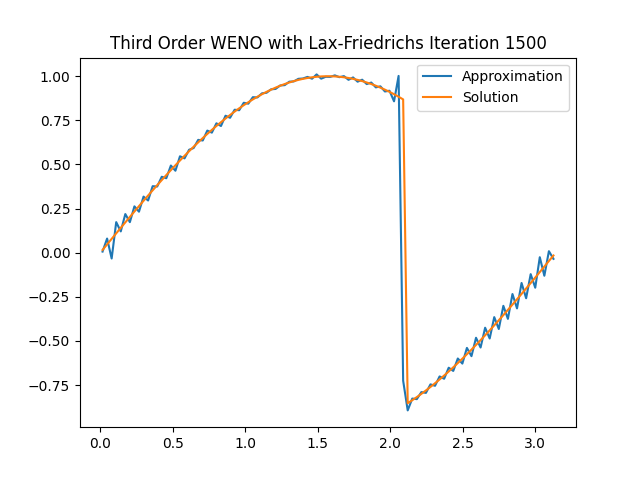
\includegraphics[width=0.9\linewidth]{imgs/output_weno3_lf/plot_1500.png}
        %   \caption{figure}{Another figure}
        % \label{fig:test2}
    \end{minipage}
\caption{Progression of the third order WENO with Lax-Friedrichs method. The method approaches a noisy approximation of the true solution and then diverges if one does not halt the convergence. The errors start to the left of the jump and propagate from there. Look closely at the 500th iteration.}
\end{figure*}
\newpage
\subsection{First order Lax–Friedrichs WENO sweeping method}
This method also diverges after a bit, however the noise starts at the singularity as opposed to the left of the singularity.
\begin{figure*}[t!]
    \centering
    \begin{minipage}{.48\textwidth}
        \centering
        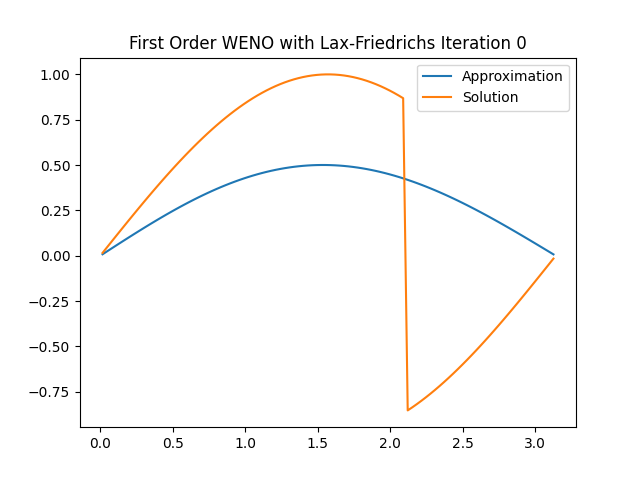
\includegraphics[width=0.9\linewidth]{imgs/output_weno1_lf/plot_0.png}
        %   \caption{figure}{A figure}
        % \label{fig:test1}
    \end{minipage}%
    \begin{minipage}{.48\textwidth}
        \centering
        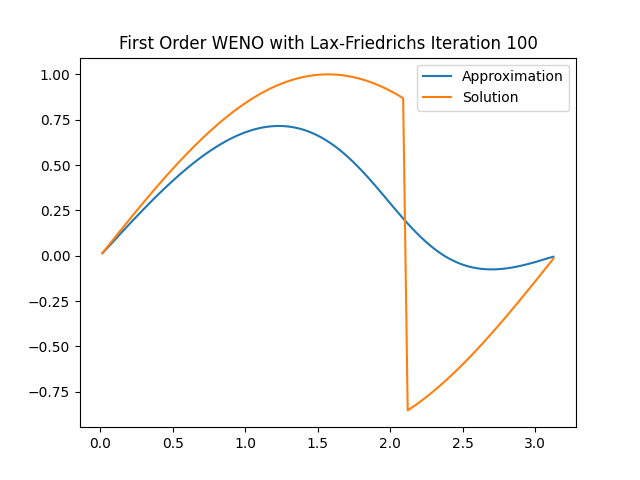
\includegraphics[width=0.9\linewidth]{imgs/output_weno1_lf/plot_100.png}
        %   \caption{figure}{Another figure}
        % \label{fig:test2}
    \end{minipage}
\par\bigskip
    \begin{minipage}{.48\textwidth}
        \centering
        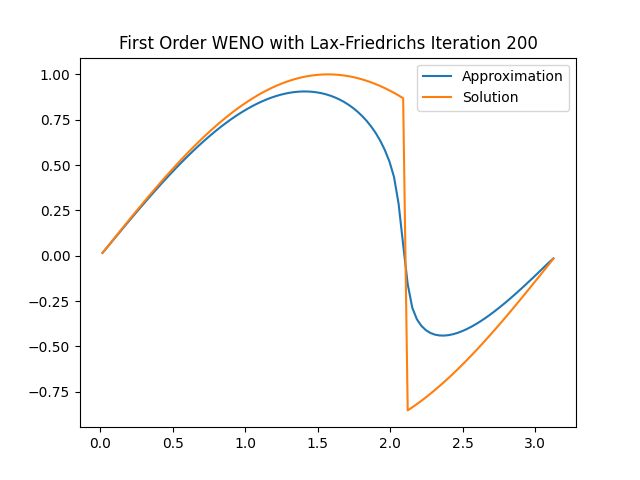
\includegraphics[width=0.9\linewidth]{imgs/output_weno1_lf/plot_200.png}
        %   \caption{figure}{A figure}
        % \label{fig:test1}
    \end{minipage}%
    \begin{minipage}{.48\textwidth}
        \centering
        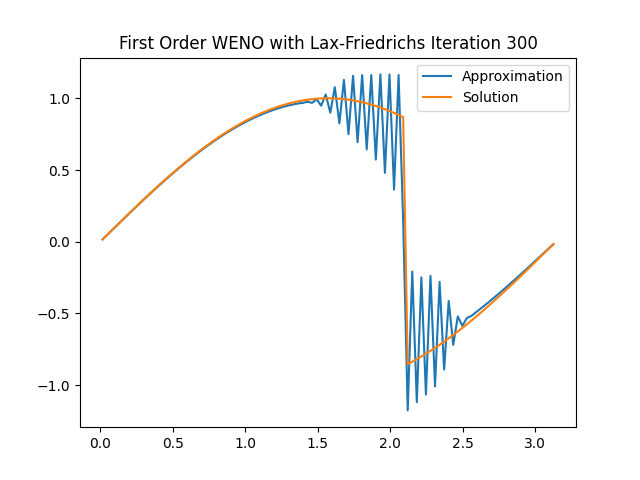
\includegraphics[width=0.9\linewidth]{imgs/output_weno1_lf/plot_300.png}
        %   \caption{figure}{Another figure}
        % \label{fig:test2}
    \end{minipage}
\caption{Progression of the first order WENO with Lax-Friedrichs method.}
\end{figure*}
\end{document}